%\documentclass[11pt, draft, oneside]{report}
\documentclass[11pt]{report}
\makeindex
\usepackage{ngerman,a4,showidx} %index an seite
%\usepackage{ngerman,a4wide}
%for pdfLaTeX output Bilder als .png speichern:
\usepackage{listings}
\usepackage{nomencl}
\usepackage{framed,color}
\usepackage[pdftex]{graphicx}
% fuer "Excel"Graphen direkt in Latex
\usepackage{pgfplots}
% f\"{u}r normales LaTeX->dvi, Bilder als .eps speichern:
\usepackage{graphicx} \DeclareGraphicsExtensions{.eps} %\graphicspath{{bilder/eps/}}

%Definition der Seitengr"osse
\setlength{\textwidth}{15 true cm}
\setlength{\textheight}{22 true cm}
\oddsidemargin  0.5 cm
\evensidemargin 0.5 cm
\topmargin      0 cm

\selectlanguage{german}
%Beispiel fuer ein neues LaTex Kommando
%\newcommand{\QSIM}{{\sc QSim}}


\begin{document}

\begin{titlepage}
\begin{center}
  \vspace*{0.5cm}
  {\LARGE Laborprotokoll Raumakustik LU - Gruppe 4} \\
  \vspace{15mm}
  {\huge \bf Labortag 1 - Messung der Nachhallzeit \\}

  \vspace{15mm}
  {\LARGE Andreas Johann H\"ormer\\
Benjamin Stahl} \\

  \vspace{10mm}%15
  -------------------------------------- \\
  \vspace{10mm}%15
  \large
  Institute for signal processing and speech communication \\
  Graz University of Technology \\


  %Vorstand: O.\,Univ.-Prof.\,Dipl.-Ing.\,Dr.\,techn.\,Reinhold Wei{\ss} \\
  \vspace{15mm}%1
  \begin{figure}[!ht]
  \begin{center}
  \centerline{
\includegraphics[width=4cm,keepaspectratio=true]{TULogoneu}}
  \end{center}
  \end{figure}
  \vspace{10mm}
Laborbetreuung: DI\,Dr.\,techn. Franz Graf \\
  %Begutachter: O.\,A.o.Univ.-Prof.\,Dipl.-Ing.\,Dr.\,techn.\,Eugen Brenner \\
  %\vspace{5mm}
  %Betreuer: Univ.-Ass. Dipl.-Ing.\,Dr.\,techn.\,N. N.\\
  \vfill
  %\newline
  %\normalsize
  Tonstudio TU Graz, 27.04.2015
  \vspace{0.5cm}
\end{center}
\end{titlepage}

% Die Titelseite ist immer in Deutsch (austrian), danach h\"{a}ngt es von der
% Sprache der Diplomarbeit ab. Jedenfalls muss eine Kurzfassung und
% ein Abstract existieren

%\thispagestyle{empty} 
%\selectlanguage{english}


\newpage
\selectlanguage{german}
%\vspace*{2.2 cm}
%{\Large
%\noindent
%{\bf Abstract}} \\
%\vspace*{0.3 cm}

%\noindent
%Main target of this laboratory was the measurement of different DACs and ADCs of the fully digital mixing panel LAWO $mc^2 66$. Additionally preamplifiers of a %high quality input compared to standard inputs were measured. Measurements were done qualitatively in terms of dynamic ranges and frequency characteristics.%\\
%This report consists of 28 pages. 


%\newpage


%\selectlanguage{english}
%\vspace*{2.2 cm}
%{\Large
%\noindent
%{\bf STATUTORY DECLARATION}} \\
%\vspace*{0.3 cm}

%\noindent
%I declare that I have authored this thesis independently, that I have not used other than the declared sources / %resources, and that I have explicitly marked all material which has been quoted either literally or by content from %the used sources.
%\vspace*{0.3 cm}

%\vspace{2 cm}

%\noindent ..............................\hfill ...........................................


%\noindent date  \hfill (signature)
\renewcommand{\nomname}{List of abbreviations}
\setlength{\nomlabelwidth}{.50\hsize}
\renewcommand{\nomlabel}[1]{#1 \dotfill}
\setlength{\nomitemsep}{-\parsep}
\makenomenclature

\newpage
\selectlanguage{german}
%\newpage
%\vspace*{2.2 cm}
%{\Large
%\noindent
%{\bf Danksagung}} \\
%\vspace*{0.3 cm}
% OPTIONAL

%\noindent
%Diese Diplomarbeit wurde im (Studien)Jahr am Institut f\"{u}r
%Technische Informatik an der Technischen Universit\"{a}t Graz
%durchgef\"{u}hrt.

%\smallskip
%Danksagung an alle am Institut bzw. bei Firmen, die geholfen
%haben....

%\medskip
%Danksagung an Freunde und Freundinnen f\"{u}r das Verst\"{a}ndnis, ebenso
%den Eltern und allen sonstigen Sponsoren....

%\vspace{2 cm}

%
%\noindent Graz, im Monat Jahr \hfill Name des Diplomanden

\newpage
% Inhaltsverzeichnis
\tableofcontents  

% Tabellenverzeichnis
% OPTIONAL
%




\listoffigures 

% Abbildungsverzeichnis
% OPTIONAL
%\listoftables

%Seitennummerierung am Kopf inkl. Kapitel"uberschrift
\pagestyle{headings}

%---------------------------------------------------------------------------------------------------------
%---------------------------------------------------------------------------------------------------------

\chapter{Messung der Nachhallzeit}
Ein wichtiges Kriterium für die statischen akustischen Verhältnisse eines Raumes ist die Nachhallzeit. Da das Ohr nicht den gesamten Lautstärkebereich von 150dB wahrnehmen kann, sondern bei einer Pegeldifferenz von 60dB unmittelbar nach dem Ende eines Nutzsignals völlige Ruhe empfindet, wird in der Regel die Nachhallzeit $T_{60}$ berechnet.[REF RAUMAKUSTIK SKRIPT SPSC v5.4]  Ist das für diese Messung erforderliche SNR durch diverse Gründe nicht erreichbar, ist auch eine Messung von $T_{20}$ oder $T_{30}$ und eine Interpolation dieser Nachhallzeit auf die gesamte Dauer möglich. Die Messung der Nachhallzeit kann unter anderem mit folgenden Methoden gemessen werden:
\begin{itemize}
\item Methode des abgeschalteten Rauschens\\
Hierzu wird der Raum mit einem Rauschsignal angeregt, bis ein diffuses Schallfeld entsteht. Nach dem Abschalten der Rauschquelle wird der Pegelabfall in den gewünschten Oktav- oder Terzbändern gemessen.
\item Messung mittels Impulsschallquelle\\
Der Raum wird mittels einer Impulsschallquelle (platzender Ballon, Pistole, etc.) angeregt. Der Pegelabfall unmittelbar nach Auftreten des Impulses wird gemessen.
\end{itemize}
%---------------------------------------------------------------------------------------------------------
\section{Messung im Aufnahmeraum AR}
\subsubsection{Einf\"uhrung}
\begin{figure}[htbp]
\begin{center}
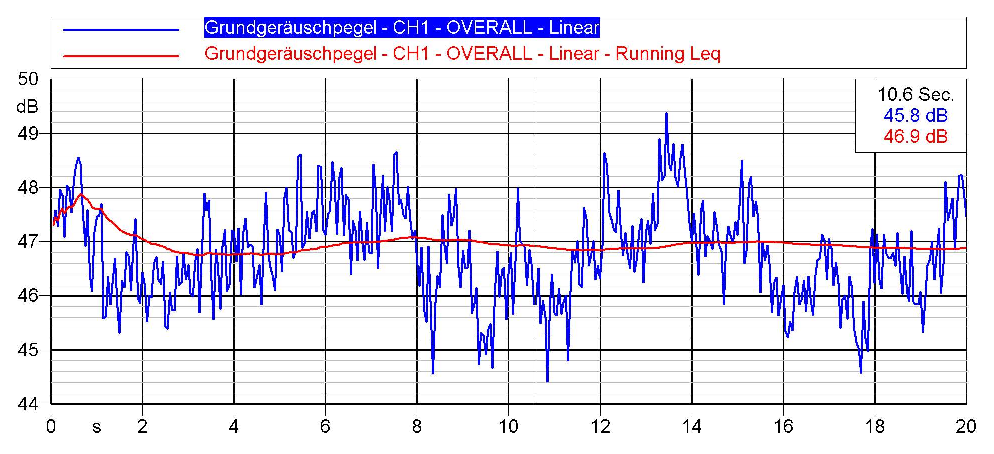
\includegraphics[width=14cm,keepaspectratio=true]{Grundrauschpegel}
\caption{Grundrauschpegel im Aufnahmeraum AR}
\label{fig:i2geometrics}
\end{center}
\end{figure}
\subsubsection{Grundlegende Berechnungen}
Die Berechnung der Mindestdistanz $d_{min}$ zwischen Schallquelle und Empf\"anger wird mit folgender Formel durchgef\"uhrt.
\begin{equation}
d_{min}=2\cdot \sqrt{\frac{V}{c\cdot T}}
\label{eq:dmin}
\end{equation}
Der Aufnahmeraum ist in Abbildung \ref{fig:ARgeometrics} ersichtlich. Das Raumvolumen ergibt sich bei gegebenen Ma\ss en zu 
\begin{equation}
V_{AR} = B\cdot T\cdot H = 5.8\,m\cdot 7.4\,m\cdot 2.88\,m = 124\,m^{3}
\end{equation}
Eine durchschnittliche Nachhallzeit wurde mittels Klatschtest gesch\"atzt und als Mittelwert $T=0.3\,s$ angenommen. Die erforderliche Mindestdistanz zwischen Rauschquelle und Mikrofon betr\"agt somit
\begin{equation}
d_{min}=2\cdot \sqrt{\frac{124\,m^{3}}{343\,\frac{m}{s}\cdot 0.3\,s}} = 2.2\,m
\end{equation}
Diese Distanz wurde bei der Wahl der Quell- und Mikrofonposition ber\"ucksichtigt, der Messaufbau in Abbildung \ref{fig:ARgeometrics} gen\"ugt dieser Bedingung.
\begin{leftbar}
\textit{ Hinweis:\\
Die Decke des Aufnahmeraums ist in zwei unterschiedlichen H\"ohen abgesetzt. Zur Berechnung des Raumvolumens wurde eine mittlere Deckenh\"ohe mit $H=\frac{H_{min}+H_{max}}{2}$ approximiert. Im Raum befindliche Objekte (Tische, Fl\"ugel, etc.) wurden nicht ber\"ucksichtigt. Das berechnete Raumvolumen ist daher etwas gr\"o\ss er als das tats\"achliche, wodurch das berechnete $d_{min}$ ebenfalls einen etwas h\"oheren Wert aufweist.} 
\end{leftbar}
%---------------------------------------------------------------------------------------------------------
%---------------------------------------------------------------------------------------------------------
\subsection{Messung mittels Methode des abgeschalteten Rauschens}



\subsubsection{Experimenteller Aufbau}
Die Messkette zur Messung der Nachhallzeit mit abgeschaltetem Rauschen ist in Abbildung \ref{fig:rauschaufbau} dargestellt.
\begin{figure}[htbp]
\begin{center}
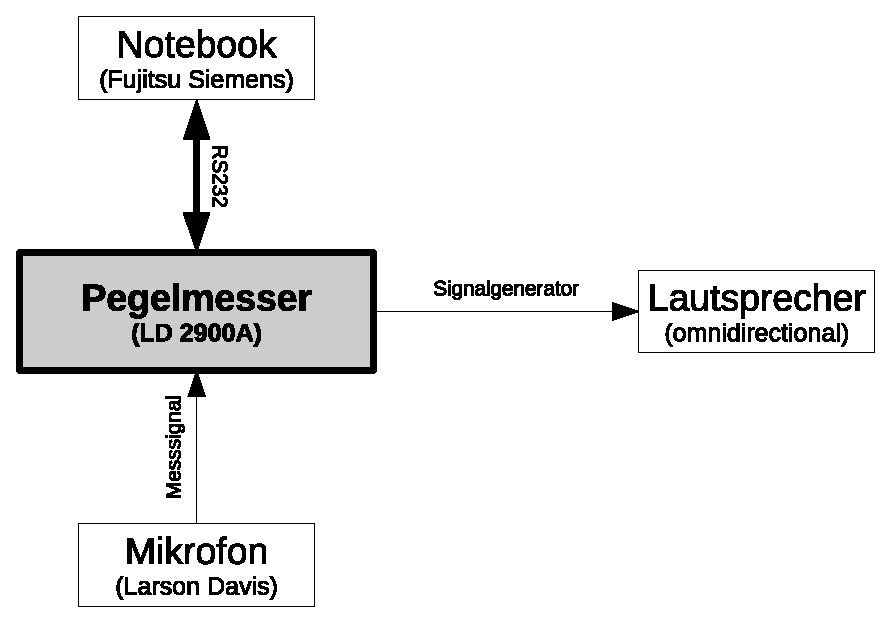
\includegraphics[width=10cm,keepaspectratio=true]{rauschaufbau}
\caption{Messkette Methode des abgeschalteten Rauschens}
\label{fig:rauschaufbau}
\end{center}
\end{figure}
\paragraph{Verwendetes Equipment}
\begin{itemize}
\item Messmikrofon: Larson Davis PRM900B3562
\item Verst\"arker: Norsonic Nor280
\begin{itemize}
\item SerNr: 280 4052
\item TU Graz InventarNr: 0103547
\end{itemize}
\item Pegelmesser: LD 2900A
\begin{itemize}
\item SerNr: 551
\end{itemize}
\item Omnidirektionaler Lautsprecher mit 12 Chassis
\begin{itemize}
\item TU Graz InventarNr: 0138945
\end{itemize}
\end{itemize}
des Weiteren:
\begin{itemize}
\item Distanzmesser: Bosch DLE70
\begin{itemize}
\item SerNr: 009634346
\item TU Graz InventarNr: 0103547
\end{itemize}
\item Fujitso Siemens Notebook
\item Kalibrator: Br\"uel\,\&\,Kj\ae r 94dB@1kHz
\end{itemize}

\paragraph{Messbedingungen}
Die Geometrien des Aufnahmeraums sind in Abbildung \ref{fig:ARgeometrics} ersichtlich. Der Raum wurde in unbesetztem Zustand vermessen. Der Fu\ss boden besteht aus filz\"ahnlichem Material, die W\"ande sind f\"ur die Messung mit schwarzen Vorh\"angen abgedeckt. Die L\"uftungsanlage ist f\"ur die Dauer der Messung deaktiviert, die T\"ure zum Regieplatz 2 (RP2) vollst\"andig geschlossen. Da das geeichte Spezialkabel zur Verbindung von Messmikrofon und Pegelmesser durch die T\"ure zum Regieplatz 1 (RP1) gef\"uhrt wird, ist diese T\"ure nur angelehnt.\\
Die Messung wurde bei einer Temperatur von $22,6^\circ C $ und einer relativen Luftfeuchtigkeit von $56,1\;rel\%$ durchgef\"uhrt.
\begin{figure}[htbp]
\begin{center}
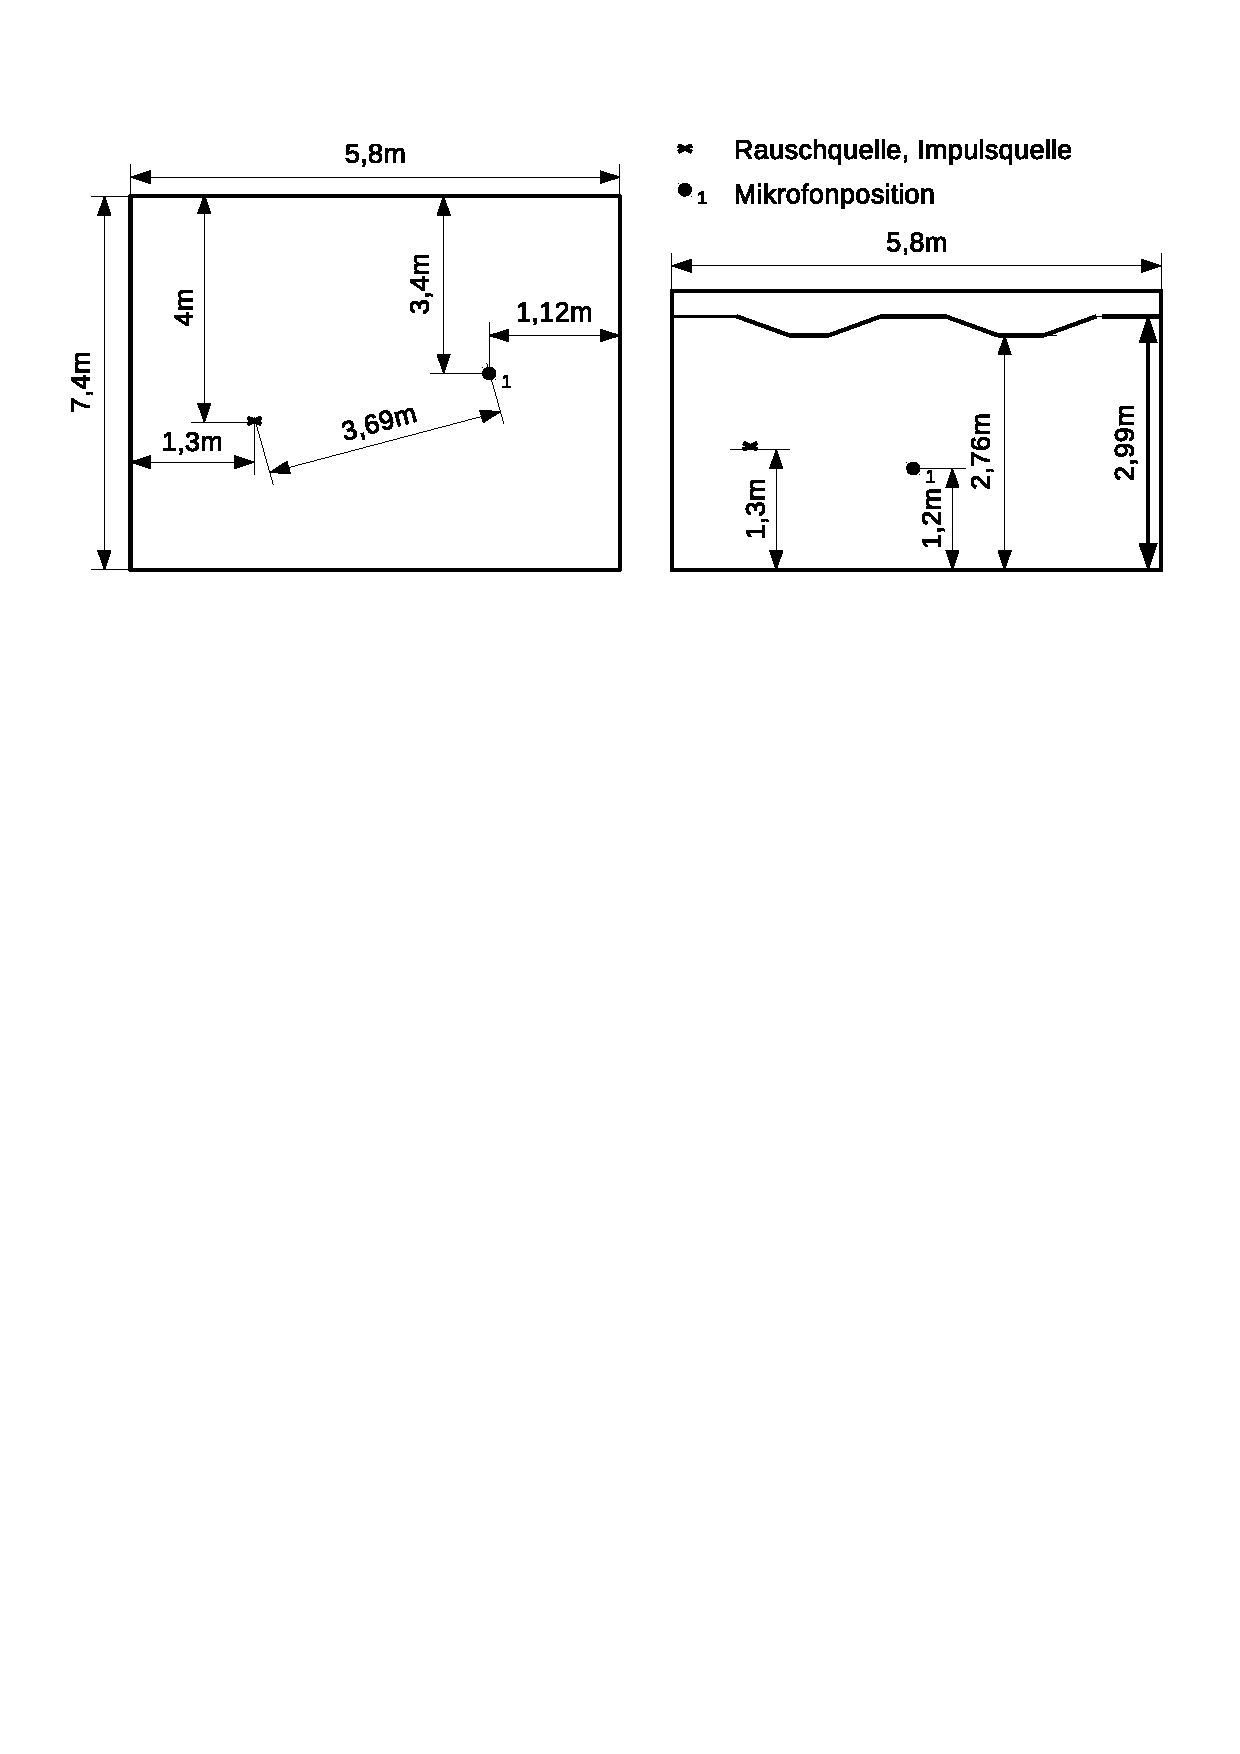
\includegraphics[width=14cm,keepaspectratio=true]{AR}
\caption{Experimenteller Messaufbau im Aufnahmeraum (links: Grundriss; rechts: Seitenriss)}
\label{fig:ARgeometrics}
\end{center}
\end{figure}
\subsubsection{Messergebnisse}
\begin{figure}[htbp]
\begin{center}
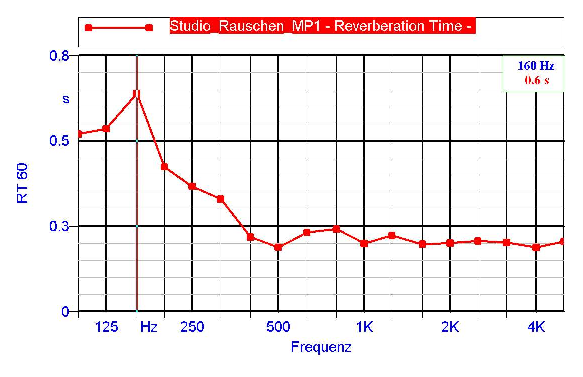
\includegraphics[width=14cm,keepaspectratio=true]{RauschenMP1}
\caption{Nachhallzeit nach Berechnung mit abgeschaltetem Rauschen (Aufnahmeraum AR)}
\label{fig:i2geometrics}
\end{center}
\end{figure}
%---------------------------------------------------------------------------------------------------------
%---------------------------------------------------------------------------------------------------------
\subsection{Impulsmessung}
\subsubsection{Einf\"uhrung}
\label{Impulseinfuehrung}
\subsubsection{Experimenteller Aufbau}
Die Messkette zur Messung der Nachhallzeit mittels Impulsschallquelle ist in Abbildung \ref{fig:impulsaufbau} dargestellt.
\begin{figure}[htbp]
\begin{center}
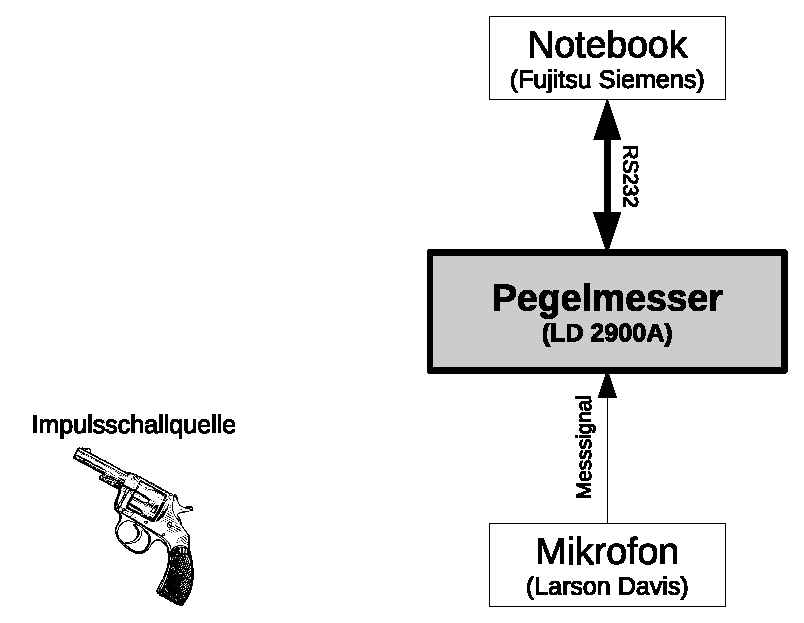
\includegraphics[width=8cm,keepaspectratio=true]{impulsaufbau}
\caption{Messkette Nachhallzeitmessung mittels Impulschallquelle}
\label{fig:impulsaufbau}
\end{center}
\end{figure}
\paragraph{Verwendetes Equipment}
\begin{itemize}
\item Messmikrofon: Larson Davis PRM900B3562
\item Pegelmesser: LD 2900A
\begin{itemize}
\item SerNr: 551
\end{itemize}
\item Gasdruckpistole ATAK Arms Ltd ZORAKI.R1
\begin{itemize}
\item SerNr: 10.14
\end{itemize}
\end{itemize}
\paragraph{Messbedingungen}
Die Messbedingungen entsprechen im Wesentlichen jenen der Messmethode mit abgeschaltetem Rauschen. Abweichend von diesen war bei dieser Messung eine Person als Impulsgeber im Raum anwesend.
\subsubsection{Messergebnisse}
\begin{figure}[htbp]
\begin{center}
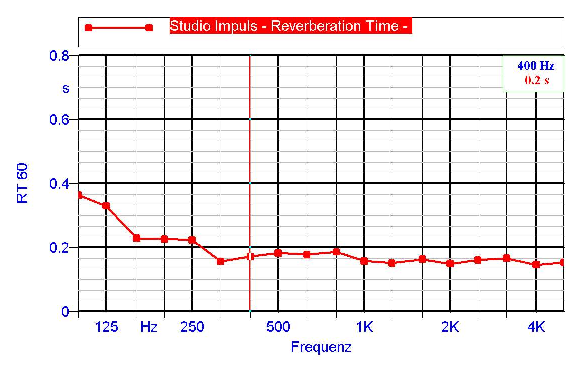
\includegraphics[width=14cm,keepaspectratio=true]{ImpulsMP1}
\caption{Nachhallzeit nach Berechnung mit Impulsschallquelle (Aufnahmeraum AR)}
\label{fig:i2geometrics}
\end{center}
\end{figure}
%---------------------------------------------------------------------------------------------------------
%---------------------------------------------------------------------------------------------------------
\section{Messung im H\"orsaal i2}
\subsection{Impulsmessung}
\subsubsection{Einf\"uhrung}
Die theoretischen Grundlagen entsprechen jenen in Kapitel \ref{Impulseinfuehrung}.
\subsubsection{Grundlegende Berechnungen}
Die Berechnung der Mindestdistanz $d_{min}$ erfolgt mit Formel \ref{eq:dmin}. Eine ungef\"ahre Nachhallzeit wurde mittels Klatschen gesch\"atzt und als durchschnittlich $T=1.2s$ angenommen. Das Raumvolumen ergibt sich nach folgender Berechnung.
\begin{equation}
V_{i2}=\Big[7.4m\cdot4.1m+1.5m\cdot2.8m+(16m-7.4m-1.5m)\cdot\frac{2.8m+4.1m}{2}\Big]\cdot10.2m
\end{equation}
\begin{equation}
V_{i2}= 602\,m^{3}
\end{equation}
Eine minimale Distanz $d_{min}$ zwischen Impulsschallquelle und Mikrofon ergibt sich durch Berechnung mit folgender Formel.
\begin{equation}
d_{min}=2\cdot\sqrt{\frac{602\,m^{3}}{343\frac\,{m}{s}\cdot 1.2s}}=2.42\,m
\end{equation}
\begin{leftbar}
\textit{ Hinweis:\\
Volumenseinbu\ss en durch Einbauten wie Tische oder Bestuhlung sowie das Volumen des im Raum eingebauten Regieraums wurden f\"ur die Volumensberechnung nicht ber\"ucksichtigt. Die berechnete Mindestdistanz ist daher geringf\"ugig gr\"o\ss er als das Optimum.}
\end{leftbar}
\subsubsection{Experimenteller Aufbau}
\paragraph{Verwendetes Equipment}
\begin{itemize}
\item Pegelmesser (handheld): NTi XL2
\begin{itemize}
\item TU Graz InventarNr: 0104784
\end{itemize}
\item Messmikrofon: NTi M4260
\begin{itemize}
\item SerNr: 1460
\end{itemize}
\item Gasdruckpistole ATAK Arms Ltd ZORAKI.R1
\begin{itemize}
\item SerNr: 10.14
\end{itemize}
\end{itemize}
\paragraph{Messbedingungen}
Die Geometrien des H\"orsaals i2 sind in Abbildung \ref{fig:i2geometrics} ersichtlich. Der H\"orsaal wird in unbesetztem Zustand vermesssen. Zum Zeitpunkt der Messung sind im Raum zwei Personen anwesend. Der H\"orsaal ist mit filz\"ahnlichem Bodenbelag sowie akustischen Lochplatten an den W\"anden ausgestattet. Die T\"uren sind w\"ahrend des Messvorgangs geschlossen. Die Messung wurde bei einer Temperatur von $23^\circ C$ und einer relativen Luftfeuchtigkeit von $43,3rel\%$ durchgef\"uhrt. 
\begin{figure}[htbp]
\begin{center}
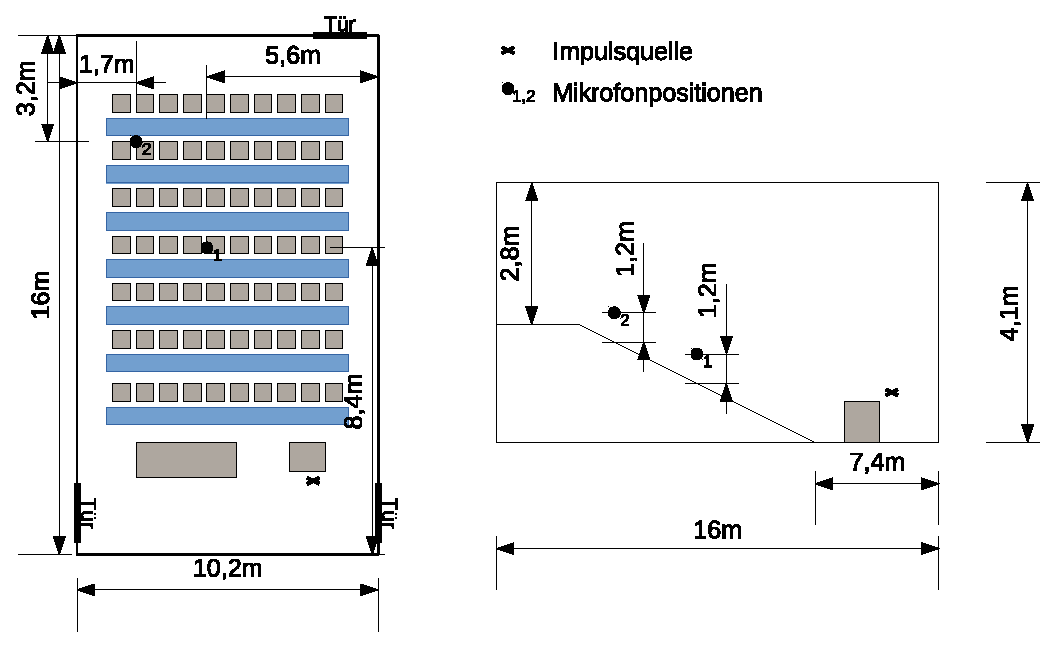
\includegraphics[width=14cm,keepaspectratio=true]{i2}
\caption{Experimenteller Messaufbau im i2 (links: Grundriss; rechts: Seitenriss)}
\label{fig:i2geometrics}
\end{center}
\end{figure}
\subsubsection{Messergebnisse}
\begin{center}
\pgfplotsset{width=14cm}
\begin{tikzpicture}
\begin{semilogxaxis}[title={$RT_{60}$ H\"orsaal i2}, xlabel={Frequenz}, ylabel={Nachhallzeit}, grid=both]
\addplot table {MP1.csv};
\addplot table {MP2.csv};
\legend{{Messpunkt 1}, {Messpunkt 2}}
\end{semilogxaxis}
\end{tikzpicture}
\end{center}



%\begin{table}
%\begin{center}
%\begin{tabular}{|c||c|c|}
%\hline 
%output channel  & 	output level [$dB_{FS}$]&		input level [$dB_u$]\\ \hline
%line out ch.24 (AR) &	-18 &	+6\\
%line out ch.24 (RP1) &	-18 &		+6\\
%HQ monitor ch.6 &	-9 		& +6\\
%phones ch.4 &	-15 &	+6\\
%\hline
%\end{tabular}
%\caption{values for output and input levels for DAC measurements}
%\label{tab:dacvalues}
%\end{center}
%\end{table}
%\begin{leftbar}
%\textit{ Note:\\
%A measurement of phase shifts is not possible when driving the system with a digital output signal.}
%\end{leftbar}

\end{document}
